\documentclass[12pt]{article}
\usepackage[utf8]{inputenc}
%\usepackage[T1]{fontenc}
%\usepackage{dejavu}
\usepackage{enumitem}

\usepackage{listings}
\usepackage{amsfonts}
\usepackage{fancyhdr}
\usepackage{comment}
\usepackage{graphicx}
\usepackage[letterpaper, top=2.5cm, bottom=2.5cm, left=2.2cm, right=2.2cm]{geometry}
\usepackage[spanish]{babel}
%\renewcommand{\item}[1]{\item \textbf{#1}}
\begin{document}

\begin{center}
%\includegraphics{logo_unah.png}\\
\bfseries{Universidad Nacional Autónoma de Honduras}\\
Facultad de Ingeniería\\
Departamento de Ingeniería en Sistemas\\
\bigskip
\bigskip
Asignatura: IS-611 Redes de Datos 2\\
Impartida  por José Mario López
\end{center}
\begin{center}
\noindent\rule{\textwidth}{1pt}
\huge{Examen II Parcial - Enrutamiento dinámico}\\
\vspace{10px}
\small{Resolución de problemas}
\noindent\rule{\textwidth}{1pt}
\end{center}

%\title{Resumen sobre Spanning-Tree Protocol}
 %\author{José Mario López}
 %\date{\today}
%\maketitle
\section{Introducción} 
Una de las tareas fundamentales en redes de datos es poder llevar un seguimiento de los problemas que presenta la topología y documentar la solución dada. Sin duda, es una buena experiencia para el estudiante de ingeniería afinar su habilidad para resolver problemas y poder establecer un esquema de trabajo para tal fin.

\section{Antes de empezar}
Se presenta una topología conformada por dos zonas. Cada zona está configurada con un protocolo de enrutamiento dinámico, como indica la figura en la siguiente página. OBS: las preguntas planteadas requieren respuesta. Haga sus anotaciones, al finalizar el examen tómeles una fotografía y adjúntela al examen. 

\begin{figure}[h]
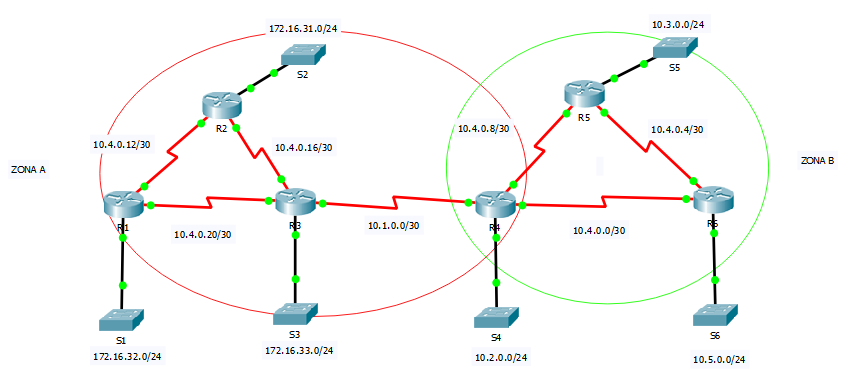
\includegraphics[scale=0.8]{img_ex2p.PNG}
\end{figure}

\section{Actividades a desarrollar (valor del examen: 15pts.)}
\subsection{Exploración de la topología}
Verifique el direccionamiento en la topología. Si hace falta alguna dirección IP o está incorrecta, configúrela correctamente.úrela correctamente.
\subsection{Configuraciones básicas}
\begin{enumerate}[label=\Alph*]
\item Añada un host a cada red. Configure el direccionamiento y verifique la conectividad entre LAN. ¿Hay conectividad total exitosa?
\end{enumerate}
\textit{\textbf{Si los mensajes en consola le dificultan la escritura de comandos, recuerde que configurar logging synchronous le ayuda evitar que los mensajes en consola interfieran con la escritura de comandos}} 

\subsection{Configuraciones}
\subsubsection{Respecto a \textbf{EIGRP} (5\%)}
\begin{enumerate}
\item Habilite EIGRP con AS 90 en la Zona A
\end{enumerate}

\subsubsection{Respecto a \textbf{OSPF} (5\%)}
\begin{enumerate}
\item Habilite OSPF con ID 100 en la Zona B
\end{enumerate}

\subsubsection{Configuración de redistribución de rutas (3\%)}
\begin{enumerate}
\item ¿En qué router se debe realizar la redistribución de rutas? Configure la redistribución y compruebe conectividad total
\end{enumerate}

\textit{\textbf{Asegúrese de guardar las configuraciones en cada router, y guardar el archivo de packet tracer.}}

\subsection{Preguntas adicionales (2\%)}
\begin{enumerate}
\item ¿Qué sucede si configuramos una ruta en EIGRP pero en vez de la wildcard usamos la máscara de subred? \#sugerencia: vea show ip protocols o show running-config
\item Referente a la topología: elimine el enlace serial entre R4 y R5. Espere unos segundos. ¿Tiene R1 una ruta para alcanzar los host de la red 10.3.0.0/24?
En caso de tenerla, ¿Cuál es su métrica? ¿Cuál es la distancia administrativa con la que fue marcada la ruta?
\end{enumerate}

\vfill
21 de agosto de 2018\\
José Mario López\\
\textit{Profesor de la asignatura}
\end{document}